% Created by tikzDevice version 0.12.3.1 on 2022-04-28 16:23:02
% !TEX encoding = UTF-8 Unicode
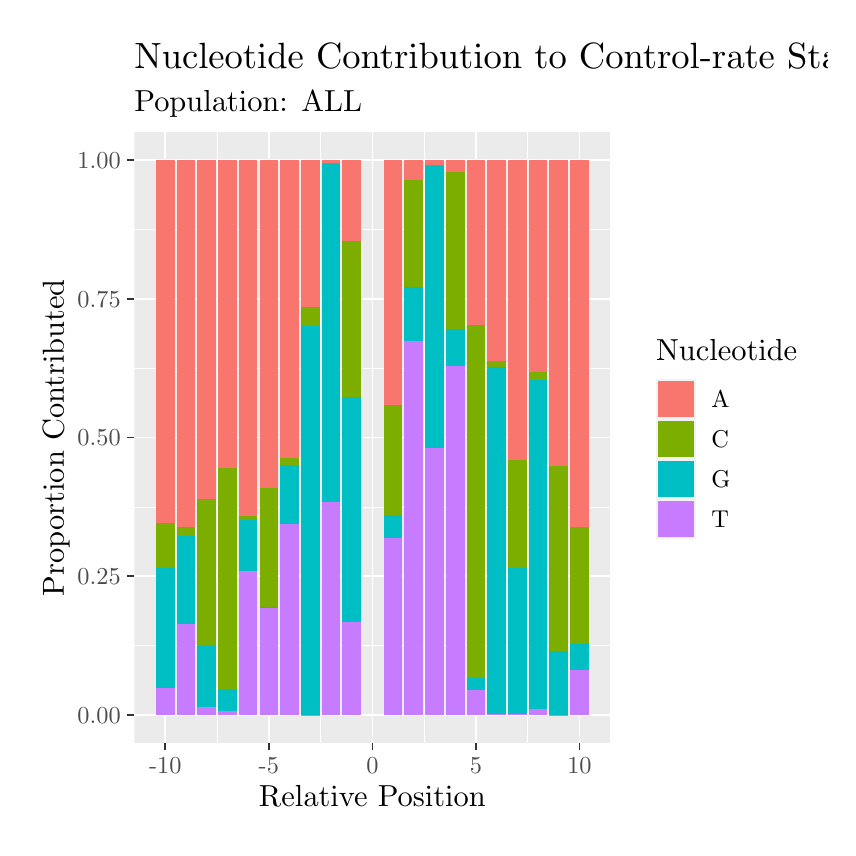
\begin{tikzpicture}[x=1pt,y=1pt]
\definecolor{fillColor}{RGB}{255,255,255}
\path[use as bounding box,fill=fillColor,fill opacity=0.00] (0,0) rectangle (289.08,289.08);
\begin{scope}
\path[clip] (  0.00,  0.00) rectangle (289.08,289.08);
\definecolor{drawColor}{RGB}{255,255,255}
\definecolor{fillColor}{RGB}{255,255,255}

\path[draw=drawColor,line width= 0.6pt,line join=round,line cap=round,fill=fillColor] (  0.00,  0.00) rectangle (289.08,289.08);
\end{scope}
\begin{scope}
\path[clip] ( 38.56, 30.69) rectangle (210.56,251.21);
\definecolor{fillColor}{gray}{0.92}

\path[fill=fillColor] ( 38.56, 30.69) rectangle (210.56,251.21);
\definecolor{drawColor}{RGB}{255,255,255}

\path[draw=drawColor,line width= 0.3pt,line join=round] ( 38.56, 65.77) --
	(210.56, 65.77);

\path[draw=drawColor,line width= 0.3pt,line join=round] ( 38.56,115.89) --
	(210.56,115.89);

\path[draw=drawColor,line width= 0.3pt,line join=round] ( 38.56,166.01) --
	(210.56,166.01);

\path[draw=drawColor,line width= 0.3pt,line join=round] ( 38.56,216.13) --
	(210.56,216.13);

\path[draw=drawColor,line width= 0.3pt,line join=round] ( 68.45, 30.69) --
	( 68.45,251.21);

\path[draw=drawColor,line width= 0.3pt,line join=round] (105.85, 30.69) --
	(105.85,251.21);

\path[draw=drawColor,line width= 0.3pt,line join=round] (143.26, 30.69) --
	(143.26,251.21);

\path[draw=drawColor,line width= 0.3pt,line join=round] (180.67, 30.69) --
	(180.67,251.21);

\path[draw=drawColor,line width= 0.6pt,line join=round] ( 38.56, 40.71) --
	(210.56, 40.71);

\path[draw=drawColor,line width= 0.6pt,line join=round] ( 38.56, 90.83) --
	(210.56, 90.83);

\path[draw=drawColor,line width= 0.6pt,line join=round] ( 38.56,140.95) --
	(210.56,140.95);

\path[draw=drawColor,line width= 0.6pt,line join=round] ( 38.56,191.07) --
	(210.56,191.07);

\path[draw=drawColor,line width= 0.6pt,line join=round] ( 38.56,241.18) --
	(210.56,241.18);

\path[draw=drawColor,line width= 0.6pt,line join=round] ( 49.74, 30.69) --
	( 49.74,251.21);

\path[draw=drawColor,line width= 0.6pt,line join=round] ( 87.15, 30.69) --
	( 87.15,251.21);

\path[draw=drawColor,line width= 0.6pt,line join=round] (124.56, 30.69) --
	(124.56,251.21);

\path[draw=drawColor,line width= 0.6pt,line join=round] (161.97, 30.69) --
	(161.97,251.21);

\path[draw=drawColor,line width= 0.6pt,line join=round] (199.38, 30.69) --
	(199.38,251.21);
\definecolor{fillColor}{RGB}{248,118,109}

\path[fill=fillColor] ( 46.37,110.10) rectangle ( 53.11,241.18);
\definecolor{fillColor}{RGB}{124,174,0}

\path[fill=fillColor] ( 46.37, 93.79) rectangle ( 53.11,110.10);
\definecolor{fillColor}{RGB}{199,124,255}

\path[fill=fillColor] ( 46.37, 40.71) rectangle ( 53.11, 50.36);
\definecolor{fillColor}{RGB}{0,191,196}

\path[fill=fillColor] ( 46.37, 50.36) rectangle ( 53.11, 93.79);
\definecolor{fillColor}{RGB}{248,118,109}

\path[fill=fillColor] ( 53.86,108.49) rectangle ( 60.59,241.18);
\definecolor{fillColor}{RGB}{124,174,0}

\path[fill=fillColor] ( 53.86,105.23) rectangle ( 60.59,108.49);
\definecolor{fillColor}{RGB}{0,191,196}

\path[fill=fillColor] ( 53.86, 73.50) rectangle ( 60.59,105.23);
\definecolor{fillColor}{RGB}{199,124,255}

\path[fill=fillColor] ( 53.86, 40.71) rectangle ( 60.59, 73.50);
\definecolor{fillColor}{RGB}{248,118,109}

\path[fill=fillColor] ( 61.34,118.84) rectangle ( 68.07,241.18);
\definecolor{fillColor}{RGB}{124,174,0}

\path[fill=fillColor] ( 61.34, 65.47) rectangle ( 68.07,118.84);
\definecolor{fillColor}{RGB}{199,124,255}

\path[fill=fillColor] ( 61.34, 40.71) rectangle ( 68.07, 43.61);
\definecolor{fillColor}{RGB}{0,191,196}

\path[fill=fillColor] ( 61.34, 43.61) rectangle ( 68.07, 65.47);
\definecolor{fillColor}{RGB}{248,118,109}

\path[fill=fillColor] ( 68.82,129.86) rectangle ( 75.55,241.18);
\definecolor{fillColor}{RGB}{124,174,0}

\path[fill=fillColor] ( 68.82, 50.00) rectangle ( 75.55,129.86);
\definecolor{fillColor}{RGB}{199,124,255}

\path[fill=fillColor] ( 68.82, 40.71) rectangle ( 75.55, 42.18);
\definecolor{fillColor}{RGB}{0,191,196}

\path[fill=fillColor] ( 68.82, 42.18) rectangle ( 75.55, 50.00);
\definecolor{fillColor}{RGB}{248,118,109}

\path[fill=fillColor] ( 76.30,112.80) rectangle ( 83.04,241.18);
\definecolor{fillColor}{RGB}{124,174,0}

\path[fill=fillColor] ( 76.30,111.34) rectangle ( 83.04,112.80);
\definecolor{fillColor}{RGB}{0,191,196}

\path[fill=fillColor] ( 76.30, 92.87) rectangle ( 83.04,111.34);
\definecolor{fillColor}{RGB}{199,124,255}

\path[fill=fillColor] ( 76.30, 40.71) rectangle ( 83.04, 92.87);
\definecolor{fillColor}{RGB}{248,118,109}

\path[fill=fillColor] ( 83.78,122.68) rectangle ( 90.52,241.18);
\definecolor{fillColor}{RGB}{124,174,0}

\path[fill=fillColor] ( 83.78, 79.61) rectangle ( 90.52,122.68);
\definecolor{fillColor}{RGB}{0,191,196}

\path[fill=fillColor] ( 83.78, 79.35) rectangle ( 90.52, 79.61);
\definecolor{fillColor}{RGB}{199,124,255}

\path[fill=fillColor] ( 83.78, 40.71) rectangle ( 90.52, 79.35);
\definecolor{fillColor}{RGB}{248,118,109}

\path[fill=fillColor] ( 91.27,133.75) rectangle ( 98.00,241.18);
\definecolor{fillColor}{RGB}{124,174,0}

\path[fill=fillColor] ( 91.27,130.99) rectangle ( 98.00,133.75);
\definecolor{fillColor}{RGB}{199,124,255}

\path[fill=fillColor] ( 91.27, 40.71) rectangle ( 98.00,109.59);
\definecolor{fillColor}{RGB}{0,191,196}

\path[fill=fillColor] ( 91.27,109.59) rectangle ( 98.00,130.99);
\definecolor{fillColor}{RGB}{248,118,109}

\path[fill=fillColor] ( 98.75,188.14) rectangle (105.48,241.18);
\definecolor{fillColor}{RGB}{124,174,0}

\path[fill=fillColor] ( 98.75,181.38) rectangle (105.48,188.14);
\definecolor{fillColor}{RGB}{199,124,255}

\path[fill=fillColor] ( 98.75, 40.71) rectangle (105.48, 40.86);
\definecolor{fillColor}{RGB}{0,191,196}

\path[fill=fillColor] ( 98.75, 40.86) rectangle (105.48,181.38);
\definecolor{fillColor}{RGB}{248,118,109}

\path[fill=fillColor] (106.23,240.10) rectangle (112.96,241.18);
\definecolor{fillColor}{RGB}{124,174,0}

\path[fill=fillColor] (106.23,239.89) rectangle (112.96,240.10);
\definecolor{fillColor}{RGB}{0,191,196}

\path[fill=fillColor] (106.23,117.79) rectangle (112.96,239.89);
\definecolor{fillColor}{RGB}{199,124,255}

\path[fill=fillColor] (106.23, 40.71) rectangle (112.96,117.79);
\definecolor{fillColor}{RGB}{248,118,109}

\path[fill=fillColor] (113.71,211.94) rectangle (120.44,241.18);
\definecolor{fillColor}{RGB}{124,174,0}

\path[fill=fillColor] (113.71,155.74) rectangle (120.44,211.94);
\definecolor{fillColor}{RGB}{199,124,255}

\path[fill=fillColor] (113.71, 40.71) rectangle (120.44, 74.21);
\definecolor{fillColor}{RGB}{0,191,196}

\path[fill=fillColor] (113.71, 74.21) rectangle (120.44,155.74);
\definecolor{fillColor}{RGB}{248,118,109}

\path[fill=fillColor] (128.67,152.65) rectangle (135.41,241.18);
\definecolor{fillColor}{RGB}{124,174,0}

\path[fill=fillColor] (128.67,112.81) rectangle (135.41,152.65);
\definecolor{fillColor}{RGB}{199,124,255}

\path[fill=fillColor] (128.67, 40.71) rectangle (135.41,104.63);
\definecolor{fillColor}{RGB}{0,191,196}

\path[fill=fillColor] (128.67,104.63) rectangle (135.41,112.81);
\definecolor{fillColor}{RGB}{248,118,109}

\path[fill=fillColor] (136.16,233.93) rectangle (142.89,241.18);
\definecolor{fillColor}{RGB}{124,174,0}

\path[fill=fillColor] (136.16,195.48) rectangle (142.89,233.93);
\definecolor{fillColor}{RGB}{199,124,255}

\path[fill=fillColor] (136.16, 40.71) rectangle (142.89,175.82);
\definecolor{fillColor}{RGB}{0,191,196}

\path[fill=fillColor] (136.16,175.82) rectangle (142.89,195.48);
\definecolor{fillColor}{RGB}{248,118,109}

\path[fill=fillColor] (143.64,239.46) rectangle (150.37,241.18);
\definecolor{fillColor}{RGB}{124,174,0}

\path[fill=fillColor] (143.64,239.21) rectangle (150.37,239.46);
\definecolor{fillColor}{RGB}{0,191,196}

\path[fill=fillColor] (143.64,137.15) rectangle (150.37,239.21);
\definecolor{fillColor}{RGB}{199,124,255}

\path[fill=fillColor] (143.64, 40.71) rectangle (150.37,137.15);
\definecolor{fillColor}{RGB}{248,118,109}

\path[fill=fillColor] (151.12,236.84) rectangle (157.85,241.18);
\definecolor{fillColor}{RGB}{124,174,0}

\path[fill=fillColor] (151.12,180.11) rectangle (157.85,236.84);
\definecolor{fillColor}{RGB}{0,191,196}

\path[fill=fillColor] (151.12,166.93) rectangle (157.85,180.11);
\definecolor{fillColor}{RGB}{199,124,255}

\path[fill=fillColor] (151.12, 40.71) rectangle (157.85,166.93);
\definecolor{fillColor}{RGB}{248,118,109}

\path[fill=fillColor] (158.60,181.53) rectangle (165.34,241.18);
\definecolor{fillColor}{RGB}{124,174,0}

\path[fill=fillColor] (158.60, 54.04) rectangle (165.34,181.53);
\definecolor{fillColor}{RGB}{199,124,255}

\path[fill=fillColor] (158.60, 40.71) rectangle (165.34, 49.79);
\definecolor{fillColor}{RGB}{0,191,196}

\path[fill=fillColor] (158.60, 49.79) rectangle (165.34, 54.04);
\definecolor{fillColor}{RGB}{248,118,109}

\path[fill=fillColor] (166.08,168.74) rectangle (172.82,241.18);
\definecolor{fillColor}{RGB}{124,174,0}

\path[fill=fillColor] (166.08,166.55) rectangle (172.82,168.74);
\definecolor{fillColor}{RGB}{0,191,196}

\path[fill=fillColor] (166.08, 41.19) rectangle (172.82,166.55);
\definecolor{fillColor}{RGB}{199,124,255}

\path[fill=fillColor] (166.08, 40.71) rectangle (172.82, 41.19);
\definecolor{fillColor}{RGB}{248,118,109}

\path[fill=fillColor] (173.57,132.81) rectangle (180.30,241.18);
\definecolor{fillColor}{RGB}{124,174,0}

\path[fill=fillColor] (173.57, 93.76) rectangle (180.30,132.81);
\definecolor{fillColor}{RGB}{199,124,255}

\path[fill=fillColor] (173.57, 40.71) rectangle (180.30, 40.93);
\definecolor{fillColor}{RGB}{0,191,196}

\path[fill=fillColor] (173.57, 40.93) rectangle (180.30, 93.76);
\definecolor{fillColor}{RGB}{248,118,109}

\path[fill=fillColor] (181.05,164.63) rectangle (187.78,241.18);
\definecolor{fillColor}{RGB}{124,174,0}

\path[fill=fillColor] (181.05,161.60) rectangle (187.78,164.63);
\definecolor{fillColor}{RGB}{0,191,196}

\path[fill=fillColor] (181.05, 42.73) rectangle (187.78,161.60);
\definecolor{fillColor}{RGB}{199,124,255}

\path[fill=fillColor] (181.05, 40.71) rectangle (187.78, 42.73);
\definecolor{fillColor}{RGB}{248,118,109}

\path[fill=fillColor] (188.53,130.64) rectangle (195.26,241.18);
\definecolor{fillColor}{RGB}{124,174,0}

\path[fill=fillColor] (188.53, 63.83) rectangle (195.26,130.64);
\definecolor{fillColor}{RGB}{199,124,255}

\path[fill=fillColor] (188.53, 40.71) rectangle (195.26, 40.76);
\definecolor{fillColor}{RGB}{0,191,196}

\path[fill=fillColor] (188.53, 40.76) rectangle (195.26, 63.83);
\definecolor{fillColor}{RGB}{248,118,109}

\path[fill=fillColor] (196.01,108.68) rectangle (202.75,241.18);
\definecolor{fillColor}{RGB}{124,174,0}

\path[fill=fillColor] (196.01, 66.45) rectangle (202.75,108.68);
\definecolor{fillColor}{RGB}{199,124,255}

\path[fill=fillColor] (196.01, 40.71) rectangle (202.75, 57.14);
\definecolor{fillColor}{RGB}{0,191,196}

\path[fill=fillColor] (196.01, 57.14) rectangle (202.75, 66.45);
\end{scope}
\begin{scope}
\path[clip] (  0.00,  0.00) rectangle (289.08,289.08);
\definecolor{drawColor}{gray}{0.30}

\node[text=drawColor,anchor=base east,inner sep=0pt, outer sep=0pt, scale=  0.88] at ( 33.61, 37.68) {0.00};

\node[text=drawColor,anchor=base east,inner sep=0pt, outer sep=0pt, scale=  0.88] at ( 33.61, 87.80) {0.25};

\node[text=drawColor,anchor=base east,inner sep=0pt, outer sep=0pt, scale=  0.88] at ( 33.61,137.92) {0.50};

\node[text=drawColor,anchor=base east,inner sep=0pt, outer sep=0pt, scale=  0.88] at ( 33.61,188.04) {0.75};

\node[text=drawColor,anchor=base east,inner sep=0pt, outer sep=0pt, scale=  0.88] at ( 33.61,238.15) {1.00};
\end{scope}
\begin{scope}
\path[clip] (  0.00,  0.00) rectangle (289.08,289.08);
\definecolor{drawColor}{gray}{0.20}

\path[draw=drawColor,line width= 0.6pt,line join=round] ( 35.81, 40.71) --
	( 38.56, 40.71);

\path[draw=drawColor,line width= 0.6pt,line join=round] ( 35.81, 90.83) --
	( 38.56, 90.83);

\path[draw=drawColor,line width= 0.6pt,line join=round] ( 35.81,140.95) --
	( 38.56,140.95);

\path[draw=drawColor,line width= 0.6pt,line join=round] ( 35.81,191.07) --
	( 38.56,191.07);

\path[draw=drawColor,line width= 0.6pt,line join=round] ( 35.81,241.18) --
	( 38.56,241.18);
\end{scope}
\begin{scope}
\path[clip] (  0.00,  0.00) rectangle (289.08,289.08);
\definecolor{drawColor}{gray}{0.20}

\path[draw=drawColor,line width= 0.6pt,line join=round] ( 49.74, 27.94) --
	( 49.74, 30.69);

\path[draw=drawColor,line width= 0.6pt,line join=round] ( 87.15, 27.94) --
	( 87.15, 30.69);

\path[draw=drawColor,line width= 0.6pt,line join=round] (124.56, 27.94) --
	(124.56, 30.69);

\path[draw=drawColor,line width= 0.6pt,line join=round] (161.97, 27.94) --
	(161.97, 30.69);

\path[draw=drawColor,line width= 0.6pt,line join=round] (199.38, 27.94) --
	(199.38, 30.69);
\end{scope}
\begin{scope}
\path[clip] (  0.00,  0.00) rectangle (289.08,289.08);
\definecolor{drawColor}{gray}{0.30}

\node[text=drawColor,anchor=base,inner sep=0pt, outer sep=0pt, scale=  0.88] at ( 49.74, 19.68) {-10};

\node[text=drawColor,anchor=base,inner sep=0pt, outer sep=0pt, scale=  0.88] at ( 87.15, 19.68) {-5};

\node[text=drawColor,anchor=base,inner sep=0pt, outer sep=0pt, scale=  0.88] at (124.56, 19.68) {0};

\node[text=drawColor,anchor=base,inner sep=0pt, outer sep=0pt, scale=  0.88] at (161.97, 19.68) {5};

\node[text=drawColor,anchor=base,inner sep=0pt, outer sep=0pt, scale=  0.88] at (199.38, 19.68) {10};
\end{scope}
\begin{scope}
\path[clip] (  0.00,  0.00) rectangle (289.08,289.08);
\definecolor{drawColor}{RGB}{0,0,0}

\node[text=drawColor,anchor=base,inner sep=0pt, outer sep=0pt, scale=  1.10] at (124.56,  7.64) {Relative Position};
\end{scope}
\begin{scope}
\path[clip] (  0.00,  0.00) rectangle (289.08,289.08);
\definecolor{drawColor}{RGB}{0,0,0}

\node[text=drawColor,rotate= 90.00,anchor=base,inner sep=0pt, outer sep=0pt, scale=  1.10] at ( 13.08,140.95) {Proportion Contributed};
\end{scope}
\begin{scope}
\path[clip] (  0.00,  0.00) rectangle (289.08,289.08);
\definecolor{fillColor}{RGB}{255,255,255}

\path[fill=fillColor] (221.56, 98.93) rectangle (283.58,182.96);
\end{scope}
\begin{scope}
\path[clip] (  0.00,  0.00) rectangle (289.08,289.08);
\definecolor{drawColor}{RGB}{0,0,0}

\node[text=drawColor,anchor=base west,inner sep=0pt, outer sep=0pt, scale=  1.10] at (227.06,168.82) {Nucleotide};
\end{scope}
\begin{scope}
\path[clip] (  0.00,  0.00) rectangle (289.08,289.08);
\definecolor{fillColor}{gray}{0.95}

\path[fill=fillColor] (227.06,147.79) rectangle (241.52,162.25);
\end{scope}
\begin{scope}
\path[clip] (  0.00,  0.00) rectangle (289.08,289.08);
\definecolor{fillColor}{RGB}{248,118,109}

\path[fill=fillColor] (227.78,148.51) rectangle (240.81,161.54);
\end{scope}
\begin{scope}
\path[clip] (  0.00,  0.00) rectangle (289.08,289.08);
\definecolor{fillColor}{gray}{0.95}

\path[fill=fillColor] (227.06,133.34) rectangle (241.52,147.79);
\end{scope}
\begin{scope}
\path[clip] (  0.00,  0.00) rectangle (289.08,289.08);
\definecolor{fillColor}{RGB}{124,174,0}

\path[fill=fillColor] (227.78,134.05) rectangle (240.81,147.08);
\end{scope}
\begin{scope}
\path[clip] (  0.00,  0.00) rectangle (289.08,289.08);
\definecolor{fillColor}{gray}{0.95}

\path[fill=fillColor] (227.06,118.89) rectangle (241.52,133.34);
\end{scope}
\begin{scope}
\path[clip] (  0.00,  0.00) rectangle (289.08,289.08);
\definecolor{fillColor}{RGB}{0,191,196}

\path[fill=fillColor] (227.78,119.60) rectangle (240.81,132.63);
\end{scope}
\begin{scope}
\path[clip] (  0.00,  0.00) rectangle (289.08,289.08);
\definecolor{fillColor}{gray}{0.95}

\path[fill=fillColor] (227.06,104.43) rectangle (241.52,118.89);
\end{scope}
\begin{scope}
\path[clip] (  0.00,  0.00) rectangle (289.08,289.08);
\definecolor{fillColor}{RGB}{199,124,255}

\path[fill=fillColor] (227.78,105.14) rectangle (240.81,118.17);
\end{scope}
\begin{scope}
\path[clip] (  0.00,  0.00) rectangle (289.08,289.08);
\definecolor{drawColor}{RGB}{0,0,0}

\node[text=drawColor,anchor=base west,inner sep=0pt, outer sep=0pt, scale=  0.88] at (247.02,151.99) {A};
\end{scope}
\begin{scope}
\path[clip] (  0.00,  0.00) rectangle (289.08,289.08);
\definecolor{drawColor}{RGB}{0,0,0}

\node[text=drawColor,anchor=base west,inner sep=0pt, outer sep=0pt, scale=  0.88] at (247.02,137.54) {C};
\end{scope}
\begin{scope}
\path[clip] (  0.00,  0.00) rectangle (289.08,289.08);
\definecolor{drawColor}{RGB}{0,0,0}

\node[text=drawColor,anchor=base west,inner sep=0pt, outer sep=0pt, scale=  0.88] at (247.02,123.08) {G};
\end{scope}
\begin{scope}
\path[clip] (  0.00,  0.00) rectangle (289.08,289.08);
\definecolor{drawColor}{RGB}{0,0,0}

\node[text=drawColor,anchor=base west,inner sep=0pt, outer sep=0pt, scale=  0.88] at (247.02,108.63) {T};
\end{scope}
\begin{scope}
\path[clip] (  0.00,  0.00) rectangle (289.08,289.08);
\definecolor{drawColor}{RGB}{0,0,0}

\node[text=drawColor,anchor=base west,inner sep=0pt, outer sep=0pt, scale=  1.10] at ( 38.56,258.85) {Population: ALL};
\end{scope}
\begin{scope}
\path[clip] (  0.00,  0.00) rectangle (289.08,289.08);
\definecolor{drawColor}{RGB}{0,0,0}

\node[text=drawColor,anchor=base west,inner sep=0pt, outer sep=0pt, scale=  1.32] at ( 38.56,274.49) {Nucleotide Contribution to Control-rate Statistic: AT-CG};
\end{scope}
\end{tikzpicture}
